\documentclass[12pt,two side]{report}
\usepackage[numbers,super,sort&compress]{natbib}
\bibliographystyle{vancouver}
%%%%%%%%%%%%%%%%%%%%%%%%%%%%%%%%%%%%%%%%%%%%%%%%%%%%%%%%%%%%%%%%%%%%%%%%%%%%%
% Definitions for the title page
% Edit these to provide the correct information
% e.g. \newcommand{\reportauthor}{Timothy Kimber}

\newcommand{\reporttitle}{Background and Progress Report I-MOTION}
\newcommand{\reportauthor}{Haiyi Wang}
\newcommand{\supervisor}{Aruna Sivakumar, Jacek Pawlak, Pancham Shukla}
\newcommand{\secondmarker}{Ivan Procaccini}
\newcommand{\degreetype}{Software Engineering}

%%%%%%%%%%%%%%%%%%%%%%%%%%%%%%%%%%%%%%%%%%%%%%%%%%%%%%%%%%%%%%%%%%%%%%%%%%%%%

% load some definitions and default packages
%%%%%%%%%%%%%%%%%%%%%%%%%%%%%%%%%%%%%%%%%
% University Assignment Title Page 
% LaTeX Template
% Version 1.0 (27/12/12)
%
% This template has been downloaded from:
% http://www.LaTeXTemplates.com
%
% Original author:
% WikiBooks (http://en.wikibooks.org/wiki/LaTeX/Title_Creation)
%
% License:
% CC BY-NC-SA 3.0 (http://creativecommons.org/licenses/by-nc-sa/3.0/)
% 
%
%%%%%%%%%%%%%%%%%%%%%%%%%%%%%%%%%%%%%%%%%
%----------------------------------------------------------------------------------------
%	PACKAGES AND OTHER DOCUMENT CONFIGURATIONS
%----------------------------------------------------------------------------------------
\usepackage[a4paper,hmargin=2.8cm,vmargin=2.0cm,includeheadfoot]{geometry}
\usepackage{textpos}
\usepackage{natbib} % for bibliography
\usepackage{tabularx,longtable,multirow,subfigure,caption}%hangcaption
\usepackage{fncylab} %formatting of labels
\usepackage{fancyhdr} % page layout
\usepackage{url} % URLs
\usepackage[english]{babel}
\usepackage{amsmath}
\usepackage{graphicx}
\usepackage{dsfont}
\usepackage{epstopdf} % automatically replace .eps with .pdf in graphics
\usepackage{backref} % needed for citations
\usepackage{array}
\usepackage{latexsym}
\usepackage[pdftex,pagebackref,hypertexnames=false,colorlinks]{hyperref} % provide links in pdf

\hypersetup{pdftitle={},
  pdfsubject={}, 
  pdfauthor={},
  pdfkeywords={}, 
  pdfstartview=FitH,
  pdfpagemode={UseOutlines},% None, FullScreen, UseOutlines
  bookmarksnumbered=true, bookmarksopen=true, colorlinks,
    citecolor=black,%
    filecolor=black,%
    linkcolor=black,%
    urlcolor=black}

\usepackage[all]{hypcap}


%\usepackage{color}
%\usepackage[tight,ugly]{units}
%\usepackage{float}
%\usepackage{tcolorbox}
%\usepackage[colorinlistoftodos]{todonotes}
% \usepackage{ntheorem}
% \theoremstyle{break}
% \newtheorem{lemma}{Lemma}
% \newtheorem{theorem}{Theorem}
% \newtheorem{remark}{Remark}
% \newtheorem{definition}{Definition}
% \newtheorem{proof}{Proof}


%%% Default fonts
\renewcommand*{\rmdefault}{bch}
\renewcommand*{\ttdefault}{cmtt}



%%% Default settings (page layout)
\setlength{\parindent}{0em}  % indentation of paragraph

\setlength{\headheight}{14.5pt}
\pagestyle{fancy}
\renewcommand{\chaptermark}[1]{\markboth{\chaptername\ \thechapter.\ #1}{}} 

\fancyfoot[ER,OL]{\sffamily\textbf{\thepage}}%Page no. in the left on odd pages and on right on even pages
\fancyfoot[OC,EC]{\sffamily }
\renewcommand{\headrulewidth}{0.1pt}
\renewcommand{\footrulewidth}{0.1pt}
\captionsetup{margin=10pt,font=small,labelfont=bf}


%--- chapter heading

\def\@makechapterhead#1{%
  \vspace*{10\p@}%
  {\parindent \z@ \raggedright \sffamily
    \interlinepenalty\@M
    \Huge\bfseries \thechapter \space\space #1\par\nobreak
    \vskip 30\p@
  }}

%---chapter heading for \chapter*  
\def\@makeschapterhead#1{%
  \vspace*{10\p@}%
  {\parindent \z@ \raggedright
    \sffamily
    \interlinepenalty\@M
    \Huge \bfseries  #1\par\nobreak
    \vskip 30\p@
  }}

\allowdisplaybreaks

% load some macros
% Here, you can define your own macros. Some examples are given below.

\newcommand{\R}[0]{\mathds{R}} % real numbers
\newcommand{\Z}[0]{\mathds{Z}} % integers
\newcommand{\N}[0]{\mathds{N}} % natural numbers
\newcommand{\C}[0]{\mathds{C}} % complex numbers
\renewcommand{\vec}[1]{{\boldsymbol{{#1}}}} % vector
\newcommand{\mat}[1]{{\boldsymbol{{#1}}}} % matrix


\date{June 2024}

\begin{document}

% load title page
% Last modification: 2015-08-17 (Marc Deisenroth)
\begin{titlepage}

\newcommand{\HRule}{\rule{\linewidth}{0.5mm}} % Defines a new command for the horizontal lines, change thickness here


%----------------------------------------------------------------------------------------
%	LOGO SECTION
%----------------------------------------------------------------------------------------


\includegraphics[width = 4cm]{./figures/imperial.jpg}\\[0.5cm] 

\center % Center remainder of the page

%----------------------------------------------------------------------------------------
%	HEADING SECTIONS
%----------------------------------------------------------------------------------------

\textsc{\Large Imperial College London}\\[0.5cm] 
\textsc{\large Department of Computing}\\[0.5cm] 

%----------------------------------------------------------------------------------------
%	TITLE SECTION
%----------------------------------------------------------------------------------------

\HRule \\[0.4cm]
{ \huge \bfseries \reporttitle}\\ % Title of your document
\HRule \\[1.5cm]
 
%----------------------------------------------------------------------------------------
%	AUTHOR SECTION
%----------------------------------------------------------------------------------------

\begin{minipage}{0.4\textwidth}
\begin{flushleft} \large
\emph{Author:}\\
\reportauthor % Your name
\end{flushleft}
\end{minipage}
~
\begin{minipage}{0.4\textwidth}
\begin{flushright} \large
\emph{Supervisor:} \\
\supervisor % Supervisor's Name
\newline
\newline
\emph{Second Marker:} \\
\secondmarker %Second Marker's Name
\end{flushright}
\end{minipage}\\[4cm]


%----------------------------------------------------------------------------------------
%	FOOTER & DATE SECTION
%----------------------------------------------------------------------------------------
\vfill % Fill the rest of the page with whitespace
Submitted in partial fulfillment of the requirements for the MSc degree in
\degreetype~of Imperial College London\\[0.5cm]

\makeatletter
\@date 
\makeatother


\end{titlepage}



% page numbering etc.
\pagenumbering{roman}
\clearpage{\pagestyle{empty}\cleardoublepage}
\setcounter{page}{1}
\pagestyle{fancy}
%%%%%%%%%%%%%%%%%%%%%%%%%%%%%%%%%%%%
%--- table of contents
\fancyhead[RE,LO]{\sffamily {Table of Contents}}
\tableofcontents 

\pagenumbering{arabic}
\setcounter{page}{1}
\fancyhead[LE,RO]{\slshape \rightmark}
\fancyhead[LO,RE]{\slshape \leftmark}

%%%%%%%%%%%%%%%%%%%%%%%%%%%%%%%%%%%%
\chapter{Introduction}
\section{Motivation}
Contemporary urban system research is undergoing a profound change, which is mainly driven by the popularization of mobile technology. The inherent capabilities of mobile devices open up new avenues for data collection, allowing researchers to delve into the complexities of human behavior in urban environments. This paradigm shift highlights the need for innovative approaches to collecting and analyzing data, especially in areas such as travel patterns, time allocation, and integration of digital activities\cite{alho2022online}.\newline

The motivation for this report stems from an awareness of the changing research environment and the urgent need to address emerging challenges and opportunities in the field. Traditional methods of data collection, while valuable, often fail to capture the dynamic nature of human behavior in urban environments\cite{mccool2021app}. Leveraging mobile platforms is a promising solution that provides real-time insights into how individuals navigate physical and digital Spaces, allocate time, and perceive productivity in different contexts.
\section{Objectives}
The project outlined in the report aims to address existing gaps in mobile data collection platforms by introducing new capabilities tailored to the specific needs of Imperial's Urban Systems Lab. By developing a new mobile platform-based time use and travel data collection platform, it aims to improve the breadth and depth of data available for interdisciplinary research efforts. This effort is driven by the desire to explore new dimensions of human behavior, from the modes of transportation used to the subtle interplay between physical and digital activities.\newline

In addition, the report aims to advance theoretical understanding and practical applications in the areas of urban planning, transportation, economics and public health. The insights gained from the data collected by the proposed platform have the potential to inform policy decisions, influence the development of urban infrastructure, and help create more livable and sustainable cities.\newline

The specific objectives of the application includes:
\begin{itemize}
  \item sensing motion of the device, to support inference of mode of transport
  \item incorporation of location-based capabilities and map-matching
  \item monitoring of app usage and data consumption
  \item Rule-driven user prompt (for data verification and manual inputs)
  \item Gathering of data from the associated wearable technologies
\end{itemize}
Fundamentally, this report is born out of a deep-seated belief in the transformative power of mobile technology to revolutionize the way we study and understand urban systems. By pushing the limits of data collection capabilities and fostering interdisciplinary collaboration, we hope to gain new insights that will drive positive change in the global urban environment.\newline

The report continues with discussing the improvements and limitations of the mobile travel data collection and survey in Chapter 2. Chapter 3 demonstrates the technical components and connectives. Section 4 presents the ideas and architectures of I-MOTION Software Systems.



%%%%%%%%%%%%%%%%%%%%%%%%%%%%%%%%%%%%
\chapter{Literature Review}
\section{Overview of Traditional Survey Methods}
Traditional traffic survey methods, such as paper-based diaries and interviews, computer-assisted telephone interviews (CATI), and GPS-based methods have long been the primary means to understand and analyze traffic travel behavior\cite{alho2022online}\cite{cottrill2013future}\cite{hong2021insights}. However, these methods generally possess inherent limitations and disadvantages. They heavily rely on respondents' memory recall of travel details, often resulting in inaccurate and incomplete data\cite{hong2021insights}. Additionally, the data quality obtained through these methods is unstable due to human memory limitations and subjectivity, making it challenging to support accurate modeling and decision-making processes\cite{cottrill2013future}. Moreover, these traditional approaches often impose significant time and effort burdens on respondents leading to low participation rates and potential data bias\cite{cottrill2013future}. Although GPS loggers can automatically record the location and movements of participants, thereby providing accurate travel data, it is necessary for participants to carry an additional device and ensure its continuous operation throughout the survey period in order to avoid missing any travel information\cite{cottrill2013future}. Moreover, relying solely on GPS data does not directly yield detailed information such as trip purpose and traffic patterns, which often require additional input from participants or inference by algorithms, thus increasing the complexity of data processing \cite{hong2021insights}.

\section{Smartphone-Based Travel Survey System}
\section {Emerging Data Methodology and Classification}
\section{Introduction of Future Mobility Sensing (FMS)\cite{alho2022online}\cite{cottrill2013future}}
FMS is a platform that collects and visualizes data by using mobile sensing technology, machine learning algorithms, and user verification to accurately record and present detailed travel and activity data. The development of future mobility sensing (FMS) technology marks a major shift in the way traffic data is collected, particularly the convergence of smartphone technology with location-based data collection. FMS utilizes GPS, GSM, Wi-Fi and accelerometers to collect high-resolution objective data on travel patterns and behavior in real time. This technique not only improves the accuracy of the data, but also reduces the recall bias associated with traditional surveys.
\begin{figure}
\centering
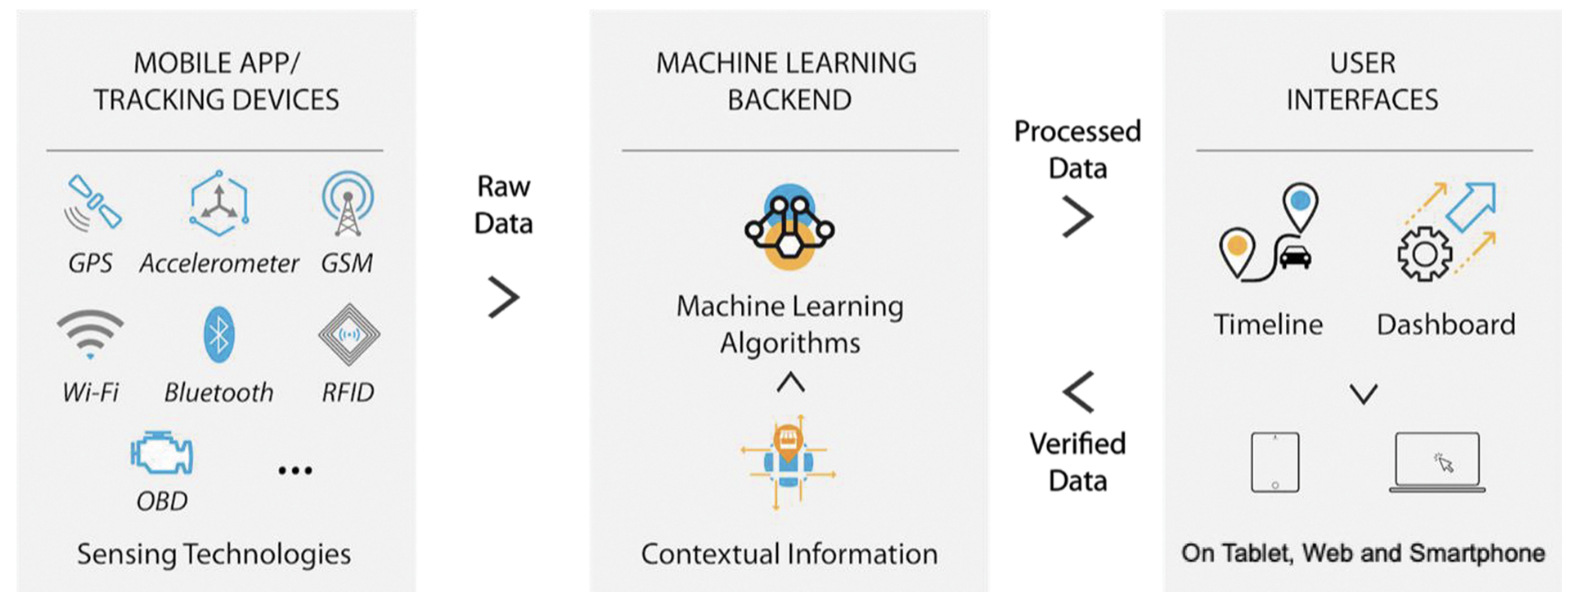
\includegraphics[width=9.1cm]{background_report/figures/FMS.png}
\caption{Future Mobility Sensing (FMS) platform architecture\cite{cottrill2013future}}
\label{figure:1}
\end{figure}
\section{Architecture of FMS}
The FMS system (Figure \ref{figure:1}) consists of three interrelated parts. It includes a mobile app or tracking device equipped with various sensing technologies to collect data\cite{cottrill2013future}. The backend of the system is a server with a database and custom algorithms to infer the details of the trip, such as the trip site, mode and purpose, thereby reducing the burden on the user\cite{cottrill2013future}. In addition, a user interface accessible through mobile phones and web platforms allows participants to verify their activities. With validation, more information can be gathered and comprehensive data can be displayed\cite{cottrill2013future}. Users can visually see their daily trips and activities on a geo-plotted timeline and can also confirm trips automatically detected by the system.
\section{Comparative Advantages of FMS}
FMS offers several distinct advantages over traditional methods. FMS is cost effective because smartphones reduce the costs associated with traditional survey methods, such as printing, mailing, and manual data entry\cite{hong2021insights}. FMS provides more accurate and details of data compared to recall-based survey. FMS uses GPS and mobile sensing to automatically record trips and details without suffering from inaccuracies of participant's memory and reduce the burden of manually recording travel details\cite{cottrill2013future}\cite{hong2021insights}. FMS captures a richer set of data, including socio-economic activities, multiple trips, and non-work-related trips\cite{hong2021insights}\cite{cottrill2013future}.  FMS is adaptable to various contexts and can be continuously improved with additional sensors and machine learning algorithms. This adaptability is crucial for capturing the rapidly changing travel behaviors, especially in response to events like the COVID-19 pandemic\cite{hong2021insights}. With the verification of participants, FMS ensures more complete data collection\cite{hong2021insights}\cite{cottrill2013future}. The user-friendly interface and automated reminders in FMS help maintain higher participant engagement and response rates compared to traditional surveys\cite{hong2021insights}. 
\section{Existing Implementations}
Over the years, many applications have been developed to fulfil the needs of smartphone-based Travel Survey. This section will delve into a few noteworthy examples that provide valuable insights into the successes and limitations associated with existing solutions.
\subsection{MoveSmarter}
The MoveSmarter smartphone application utilized by the Dutch Mobile Traffic Panel enhances the analysis of travel behavior through the utilization of automatic detection and data collection functions. It leverages smartphone sensors such as GPS, WiFi, and accelerometers to automatically identify trip start and end points, transportation modes, and trip purposes. This data is then refined through back-end processing that includes filtering and map matching techniques\cite{geurs2015automatic}. Additionally, the system incorporates a suggestive recall survey where participants can review and amend their own travel data, thereby enhancing the accuracy of collected information. This automated approach not only simplifies data collection processes and reduces respondent burden but also improves granularity and accuracy of travel data over extended periods of time through continuous tracking. Furthermore, it captures dynamic changes in travel behavior\cite{geurs2015automatic} that are challenging to capture with traditional one-time surveys.\newline


However, there are several areas where MoveSmarter can be further improved. The current app misses approximately 20-25\% of trips, particularly those with short activity durations or involving public transportation usage; thus indicating a need for enhanced trip detection capabilities\cite{geurs2015automatic}. Moreover, high battery consumption associated with applications may discourage user participation while impacting the integrity of collected data; hence necessitating better battery management strategies\cite{geurs2015automatic}. Furthermore, there is room for improvement in accurately detecting traffic patterns especially when distinguishing similar patterns like cycling versus walking or reliably identifying various forms of public transportation\cite{geurs2015automatic}.

\subsection{MEILI}
The MEILI system is an advanced platform for the automatic collection and annotation of travel diaries, designed to capture and analyze travel behavior using GPS data from multiple users. MEILI streamlines the process of collecting travel diaries by integrating GPS traces and user annotations to define trips and segments within a trip, known as "triplegs". What sets this system apart is its open-source and modular architecture, which can be customized and adjusted by researchers based on specific needs and legal requirements. The primary strength of MEILI lies in its ability to minimize manual input from participants through automated data collection and preliminary annotation, thereby enhancing data accuracy while reducing user burden. Moreover, it supports various active re-learning machine learning techniques that aid in data annotation, ultimately improving the overall efficiency of travel behavior research.\newline

However, there are several limitations with the MEILI system. Its reliance on continuous GPS tracking leads to significant battery depletion, potentially discouraging user participation. Additionally, the accuracy of automatic trip detection algorithms needs improvement, particularly for short trips and public transport modes where certain activities may not be accurately captured. Furthermore, as the number of users increases, execution time required for CRUD operations along with database capacity can become prohibitive. Recognizing these shortcomings, the authors also acknowledge that such an application should not solely focus on recording travel but should collect additional data to enable more comprehensive analysis of human mobility.
\section{Summary}
While FMS has made welcome progress in travel data collection, its implementation is not without challenges. Issues such as digital literacy among the elderly, privacy concerns, and the widespread use of smartphones are all barriers that need to be addressed. Future research could focus on improving user interfaces for seniors, strengthening data privacy protections, and integrating FMS with other data sources to create comprehensive, user-friendly mobile tracking systems.


%%%%%%%%%%%%%%%%%%%%%%%%%%%%%%%%%%%%
\chapter{Technical Preparations}
IMOTION is a complex software system with microservices, including front-end, back-end, deep learning algorithms, data management, microservices architecture management, agile development, and other requirements. As you can see in figure \ref{figure:5}, the tools required for this system are numerous and complex, and in order to make it easier to understand each tool and how they work with each other in the real world, this chapter will describe their principles and features and explain how they can play a key role in my system.
\section{Mobile Framework: Swift}

Swift is Apple's proprietary programming language designed for iOS, macOS, watchOS, and tvOS application development\cite{swift}. Known for its security features, speed, and modern syntax, it is powerful and easy for developers to use. In mobile development, Swift's performance optimizations and comprehensive error handling enable developers to build fast, reliable applications.\cite{swift} In Xcode's integrated development environment, swift development can be hot deployed and updated in real time\cite{swift}. In addition, swift has a rich set of frameworks for invoking the underlying functions of Apple devices, including GPS, gyroscopes, accelerometer, data usage detection, and inter-device communication\cite{swift}. With these capabilities, swift can provide a complex and efficient user experience for my applications.

\section{Backend Framework: Java Spring \& Python FastAPI}
The Java Spring Framework and Python FastAPI are two popular back-end frameworks today that are widely used to build high-performance and easily extensible server-side applications.\newline

Java Spring stands out for its versatility and high degree of integration, and it is suitable for the full range of development from simple stand-alone applications to complex enterprise applications\cite{SpringFramework}. Spring provides developers with a powerful and flexible programming and configuration environment that covers tasks as diverse as dependency injection, aspect oriented programming, and transaction management. Its modular design allows developers to accurately select the required components according to the needs of the project, thereby increasing the efficiency of application development\cite{SpringFramework}. In addition, Spring has a large developer community that provides rich framework support for a variety of features\cite{SpringFramework}. Spring's database connectivity capabilities, powerful security configuration capabilities, and extensive ecosystem of cloud-native microservices have made it a great convenience for me as I develop my applications.\newline

Python FastAPI is a modern API framework designed for high-performance application development. It makes clever use of Python's async/await asynchronous features, type annotations, and automated data model validation, which not only greatly reduces the amount of code, but also significantly improves runtime efficiency\cite{fastapi_website}. Because of its support for asynchronous programming, FastAPI shows excellent performance when dealing with large data volumes or high concurrency scenarios, making it particularly suitable for IO-intensive applications\cite{fastapi_website}. When I am developing machine learning services, FastAPI is able to handle the huge amount of training and prediction data with ease, which is perfect for my needs.

\section{Database: PostgreSQL \& Redis}
PostgreSQL and Redis are widely used in their respective areas of industry to build full-featured, efficient, and secure database management systems.\newline

PostgreSQL is a cutting-edge open source object-relational database system recognized for its stability, high performance, and ability to handle complex queries\cite{postgresql}. It supports a wide variety of data types and shows high scalability, enabling users to create personalized functions and data types, and to write server-side code in a variety of programming languages. PostgreSQL adheres to the ACID standard, making it a useful tool for transaction processing systems with strict data integrity requirements\cite{postgresql}. At the same time, it provides excellent concurrency support in environments with frequent read and write operations through multi-version concurrency control (MVCC) technology, thereby improving efficiency. In addition, PostgreSQL is very scalable, so it is ideal for handling large amounts of data in enterprise applications. Since the data that my application needs to store, such as latitude, speed, username, etc., relates only to the underlying data types, and there are associations between these data, a relational database becomes my first choice. At the same time, given the need for security and extensibility, PostgreSQL meets my requirements.\newline

Redis is a memory-based unstructured data storage solution that can be used as a database, cache, and message broker\cite{redis}. Redis is known for its incredible speed and supports multiple data structures such as strings, lists, collections, and ordered collections, so it can handle a variety of application scenarios from basic caching to complex messaging patterns\cite{redis}. The atomicity of its operation provides a reliable performance guarantee for concurrent data processing. While Redis primarily runs in memory to ensure its performance, it is often used for high-speed transactions and real-time applications, making it ideal for scenarios that require fast data access, such as caching, session management, and real-time analytics. In order for my application to respond quickly to user needs, I need to quickly store some hot data that does not need to be persisted, such as session information. Redis features make it ideal for achieving this goal.

\section{Machine Learning: PyTorch}
PyTorch, an open source machine learning framework developed by Facebook's AI Research Lab, stands out for its dynamic compute graphs, Python interface, GPU acceleration, rich ecosystem of tools and libraries, and active community\cite{pytorch}. Its dynamic computation diagrams allow for flexible model building and runtime modifications, simplifying debugging and facilitating experimentation. PyTorch integrates seamlessly with Python, simplifying development and prototyping, while significantly improving performance through CUDA's GPU acceleration\cite{pytorch}. That makes it suitable for training deep neural networks on large datasets. Its extensive ecosystem and active community provide resources and support for a variety of tasks and applications, which also help me to build my own deep learning model for my application.

\section{Distributed microservice Framework: Docker\& Kubernetes}
Kubernetes, referred to as K8s, is a Google-developed open-source orchestration platform for containers. It facilitates automated deployments, large-scale seamless scalability, and the proficient handling of containerized applications\cite{kubernetes_website}. Its capacity to spawn and oversee multiple containers streamlines operational and maintenance workloads, thanks to its inbuilt load balancing strategies that aid in the management, discovery, and access of application instance clusters\cite{kubernetes_website}. In the realm of microservices, Kubernetes brings forth automated deployments, scalability, and administrative abilities, which adjust the volume of service instances in real-time to accommodate fluctuating loads efficiently, all while maintaining optimal availability and minimizing resource wastage. Additionally, its clever scheduling mechanism ensures optimal resource usage by allocating resources based on the actual needs of each container and service.\newline

Docker is an open-source containerization tool that aids developers in bundling applications and their dependencies into nimble, transferable containers, ready for deployment on any widespread Linux system. Docker boasts several noteworthy features, including a secure container environment, minimal performance impact, virtualization, app isolation, and swift deployment\cite{docker_website}. In a microservices setup, Docker's containerization allows every microservice to operate independently within its own container, ensuring uninterrupted deployments and operations. This self-sufficiency bolsters the portability and responsiveness of microservices, simultaneously elevating the system's fault tolerance and scalability.\newline

When it comes to microservices, both Kubernetes and Docker are indispensable. Docker wraps up microservices in distinct containers, easing their rapid deployment and isolation. Kubernetes, meanwhile, oversees and coordinates these containers, automating deployments, scaling, load distribution, and service identification. The amalgamation of these technologies vastly simplifies the oversight and operation of microservices, boosting developmental and deployment efficiency, and guaranteeing superior durability and flexibility. This symbiotic blend enables microservices frameworks to adapt swiftly to business needs, scaling up or down as required. As a result, deploying an array of services within my server-based applications becomes a breeze, with phased introductions of new services being a straightforward endeavor.
\section{Database framework: Amazon RDS}
Amazon RDS, or Amazon Relational Database Service, is an excellent service from Amazon Cloud Technologies that minimizes the complexity and hassle of relational databases\cite{awsrds}. RDS not only provides users with an easy-to-use control panel that helps them quickly create, configure, and manage databases, but also greatly reduces the operational burden of users through automated hardware and software maintenance\cite{awsrds}. RDS supports relational database engines such as MySQL, PostgreSQL, and Oracle, regardless of business requirements. At the same time, its high-performance storage and scalable architecture ensures the efficiency and stability of the database, and the powerful data backup and recovery mechanism ensures the security of the data. RDS's real-time monitoring and alerting system gives users a comprehensive view of the health of the database, and any performance issues or anomalies can be timely feedback and dealt with\cite{awsrds}. For those features, Amazon RDB is a reliable service to store my application's data. 
\section{DevOps: Jenkins}
Jenkins plays a pivotal role in DevOps systems, orchestrating the symphony of continuous integration (CI) and continuous delivery (CD)\cite{jenkins}. It constantly monitoring changes to the code, and if there is a change, it quickly triggers the build process. This automated monitoring mechanism allows Jenkins to efficiently integrate code changes and significantly reducing integration headaches. Jenkins also moves into automated testing, executing tests with a high degree of accuracy to ensure that code quality is always at a high standard. This automation not only speeds up the feedback loop, but also reduces the risk of errors in the production environment\cite{jenkins}. Jenkins is designed in a coded way to make the process from development, staging and deployment to production smoother and more elegant. At the same time, its deep compatibility with a variety of tools and technologies has further make it important in DevOps workflows\cite{jenkins}. Its strong scalability allows developers to tailor CI/CD processes to their actual needs and adapt flexibly as needs change. The core values of DevOps in Jenkins - automation, collaboration, and continuous improvement, which can help me to build my software in a effective way.

\section{Reflection}
I opted for a microservices architecture for my application due to its potential as an open source service. This approach eliminates the added expenses associated with third-party services and avoids the creation of closed systems that cater only to limited user groups. In contrast, a monolithic application poses challenges for other researchers who wish to modify the software code, given its tightly coupled nature with numerous interconnected services and components. On the other hand, under a microservice architecture, researchers have the freedom to add or modify features without impacting the functionality of other aspects. Additionally, microservice applications offer robust stability and disaster recovery capabilities by leveraging circuit breakers and auto scaling mechanisms that dynamically adjust application size based on current demand. Furthermore, microservices enable applications to leverage multiple programming languages in areas where they are most suitable, albeit at the cost of increased complexity and a steeper learning curve; however, this trade-off results in a more flexible architectural design.

%%%%%%%%%%%%%%%%%%%%%%%%%%%%%%%%%%%%
\chapter{Project Plan}
This project develops an application named I-MOTION, a modern cloud-native distributed mobile application that revolutionaries the smartphone-based person travel survey system and extends from a pure research application to a daily healthy tracking application for growing the research population. Although this project focuses on United Kingdom, its features and functionalities can be implemented and changed in any countries in a micro-serviced way.\newline

I-MOTION provides the following features:
\begin{itemize}
  \item Real-Time Motion Trail \& Trip Timeline Prediction Demonstration: 
  
  I-MOTION can show users' trips and activites in the specific day. Users can choose to see any day of their trails by switching in the calendar.
  
  \item Background Sensors' Updating \& Predictions with No Sense:

  When users don't use this application in the foreground, the application still record telephone's sensors(GPS, accelerometer, heart readers, etc.) and frequently predict and improve the model frequently
  
  \item Smart Watch Usage \& Connectivity:

  Use smart watch to record locations and other data in the way of GPS and other sensors like heart reader and blood oxygen to track healthy info.
  
  \item Verification of Predictions:

  Although this application will predict users' type of trips like modes of transport, users can still edit these predictions to make them as accurate as possible.
  
  \item Join Families \& Friends:

  Users can join their families in their activities and trips if families are connected by unique household ID. Users can also add others outside family by typing users' ID.

  \item Statistical Summary of Analysis:
  
  Applications summarises variable aspects of users' trips weekly, monthly, yearly, such as: percentage of modes of transports, data usage, and electrical \& fuel usage at home or in cars

  \item Third-Party API Support:

  Application integrates with APIs from partners, like Octopus Energy for electrical usage, SmartCar for fuel usage.

  \item Community Ranking for Good:

    Show users' ranking of green trips with their near people or the whole nations to help them having competitions or self-management, which makes this is not just only a research app.
  
\end{itemize}
\section{Proposed Timeline}
\begin{enumerate}
    \item \textbf{Requirement Gathering \& API Development}:
    \begin{itemize}
        \item User API: May 5 - May 17
        \item Data Collection API: May 10 - May 15
        \item Researcher API: May 15 - May 21
        \item Community API: May 22 - May 23
        \item Statistics API: May 24
        \item Survey API: May 24 - May 25
        \item Machine Learning API: May 26 - May 30
    \end{itemize}
    
    \item \textbf{Microservice Development}:
    \begin{itemize}
        \item Feign Connection: May 31 - June 2
        \item Jenkins DevOps Environment Setup: June 3 - June 6
        \item Junit Automation: June 6 - June 8
        \item Pod Setup: June 9 - June 16
        \item Service Setup: June 17 - June 24
        \item Ingress Setup: June 25 - July 2
        \item Microservice Creation: July 3 - July 10
    \end{itemize}
    
    \item \textbf{Frontend Development}:
    \begin{itemize}
        \item Login/Register: July 11 - July 12
        \item Track: July 13 - July 14
        \item Statistics: July 15 - July 16
        \item Wash-U: July 17 - July 18
        \item Community: July 19 - July 20
        \item Survey: July 21 - July 22
        \item Third Party API: July 23 - July 24
    \end{itemize}
    
    \item \textbf{Testing \& Debug \& Evaluation}:
    \begin{itemize}
        \item Testing \& Final Report: July 25 - September 4
    \end{itemize}
\end{enumerate}
\section{Frontend Design}
\subsection{User Interface}
\begin{itemize}
    \item SignUp/Login/Forgot Password/Logout: Sign Up by email/phone and password and validate by code. Login with email/phone and password.
    \item Main Screen:
        \begin{itemize}
            \item Track
            \item Statistics
            \item Community
            \item Setting
            \item Survey
        \end{itemize}
\end{itemize}
\subsection{User Experience}
\begin{itemize}
    \item Simplicity: Application will run in background in the most time. Users don’t need to do anything in the most time.
    \item Interactivity: every use is easy to follow. No use threshold.
    \item Usability: Not only for research purpose, users can also get useful information for them to track their daily habit.
    \item Privacy: keep data in the good security.
\end{itemize}


\section{System Design}
\subsection{Mobile Design (Figure \ref{figure:3})}
The design of the Apple mobile app for mobile devices seamlessly integrates the mobile and watch apps, creating a comprehensive and complementary system. On the mobile side, it leverages the SwiftUI framework, a modern and declarative user interface building tool, to craft an intuitive and user-friendly interface. Simultaneously, by incorporating the MapKit framework, applications can embed detailed map views that not only facilitate location tracking but also offer extensive map functionalities. Moreover, this application utilizes the CoreMotion framework to access device data such as GPS and accelerometer information in order to provide users with precise path tracking and traffic usage prediction.\newline

The design of the watch app also utilizes the SwiftUI framework to ensure visual and interactive consistency with the mobile app, thereby enhancing user experience. The watch app tracks users' health and path information, leveraging the WatchConnectivity framework for seamless data exchange between mobile apps and watch apps. This enables key health information collected on the watch to be seamlessly transferred to the mobile app, providing users with a holistic view of their health management.\newline

The primary objective of this mobile system is to provide users with a seamless cross-device experience, allowing them to easily access and manage key functions on their mobile devices while receiving instant tracking data and notifications through the watch app. This design approach ensures that users have convenient access to relevant information and services regardless of their situation. By incorporating GPS tracking, CoreMotion data collection, and traffic forecasting functions, this application successfully combines health monitoring, path tracking, and traffic analysis capabilities to provide users with in-depth insights. The functional complementarity between these two applications provides users with a comprehensive and convenient experience. Additionally, URLSession is intelligently utilized for server data retrieval while CoreData ensures secure long-term storage within the entire system's data flow.

\begin{figure}
\centering
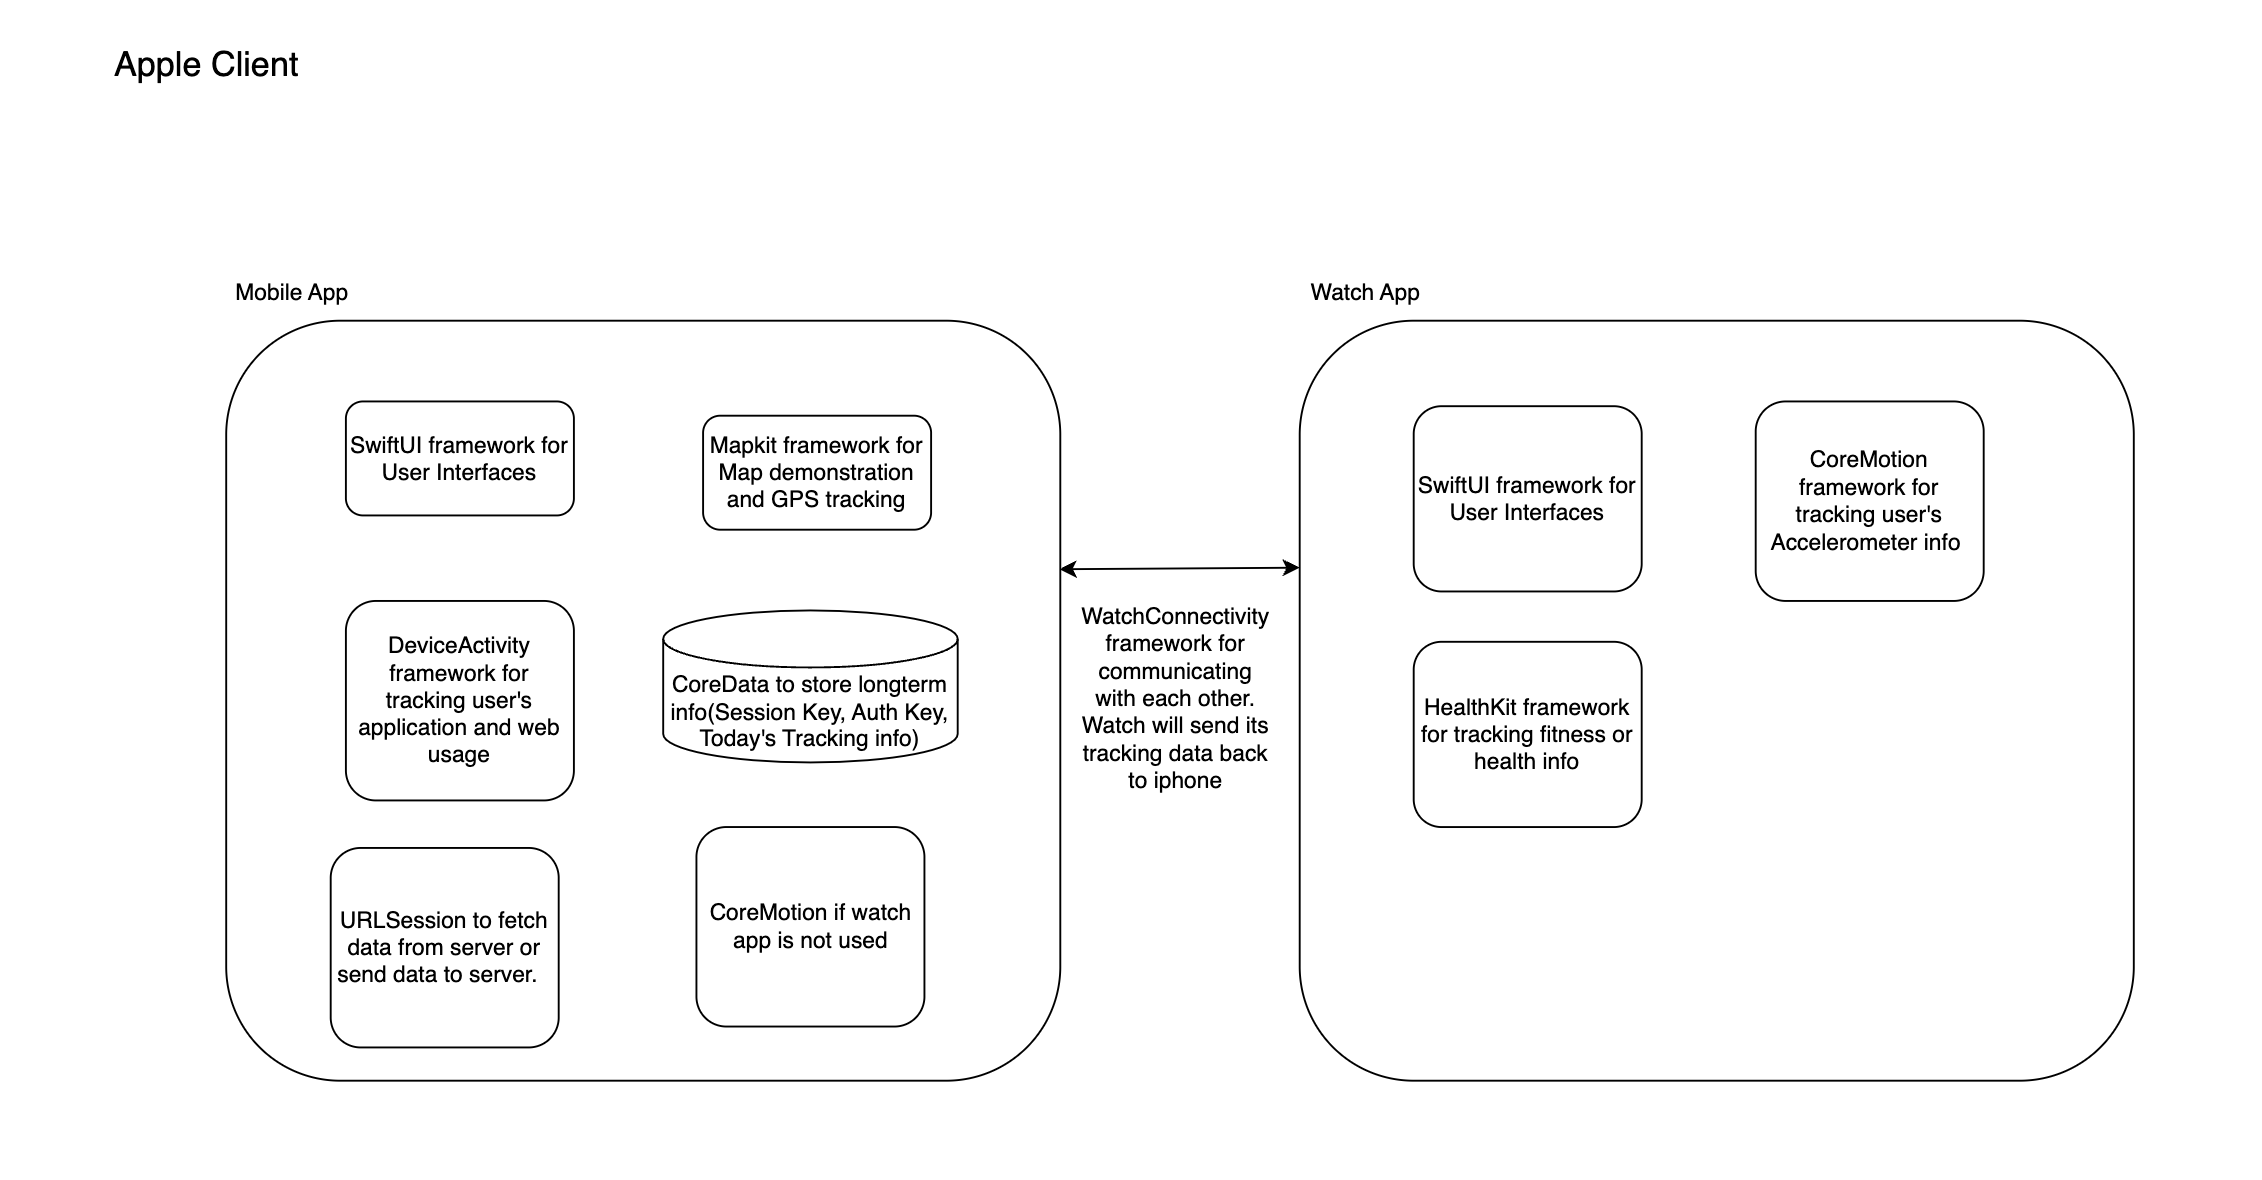
\includegraphics[width=16cm]{background_report/figures/mobile-system.png}
\caption{IMOTION Mobile System}
\label{figure:3}
\end{figure}

\subsection{Web Design (Figure \ref{figure:4})}
The Web client utilizes ReactJS to construct the user interface. ReactJS is a widely adopted front-end JavaScript library that effectively constructs responsive and interactive user interfaces, enabling researchers to manipulate and manage their data with enhanced intuitiveness. By design, the Web client offers two primary methods for handling data: JSPdf-autotable and export-from-json. The JSPdf-autotable method empowers researchers to directly convert data into PDF files, which proves valuable for those who need to generate reports or documents. Through JSPdf-autotable, researchers can personalize the appearance and layout of PDF files, ensuring precise data representation and readability. Conversely, the export-from-json method provides the flexibility to transform data into alternative formats such as XML and CSV files. This functionality is crucial for researchers seeking integration with other systems or conducting in-depth analysis. By selecting export-from-JSON, researchers can effortlessly export data in their desired format for seamless interaction with other tools or platforms. In terms of privacy settings, this Web client allows researchers to adjust the privacy level of their data according to individual requirements. Whether opting for JSPdf-autotable or export-from-json, researchers have the ability to modify privacy settings based on data sensitivity and purpose while guaranteeing utmost security and compliance.
\begin{figure}
\centering
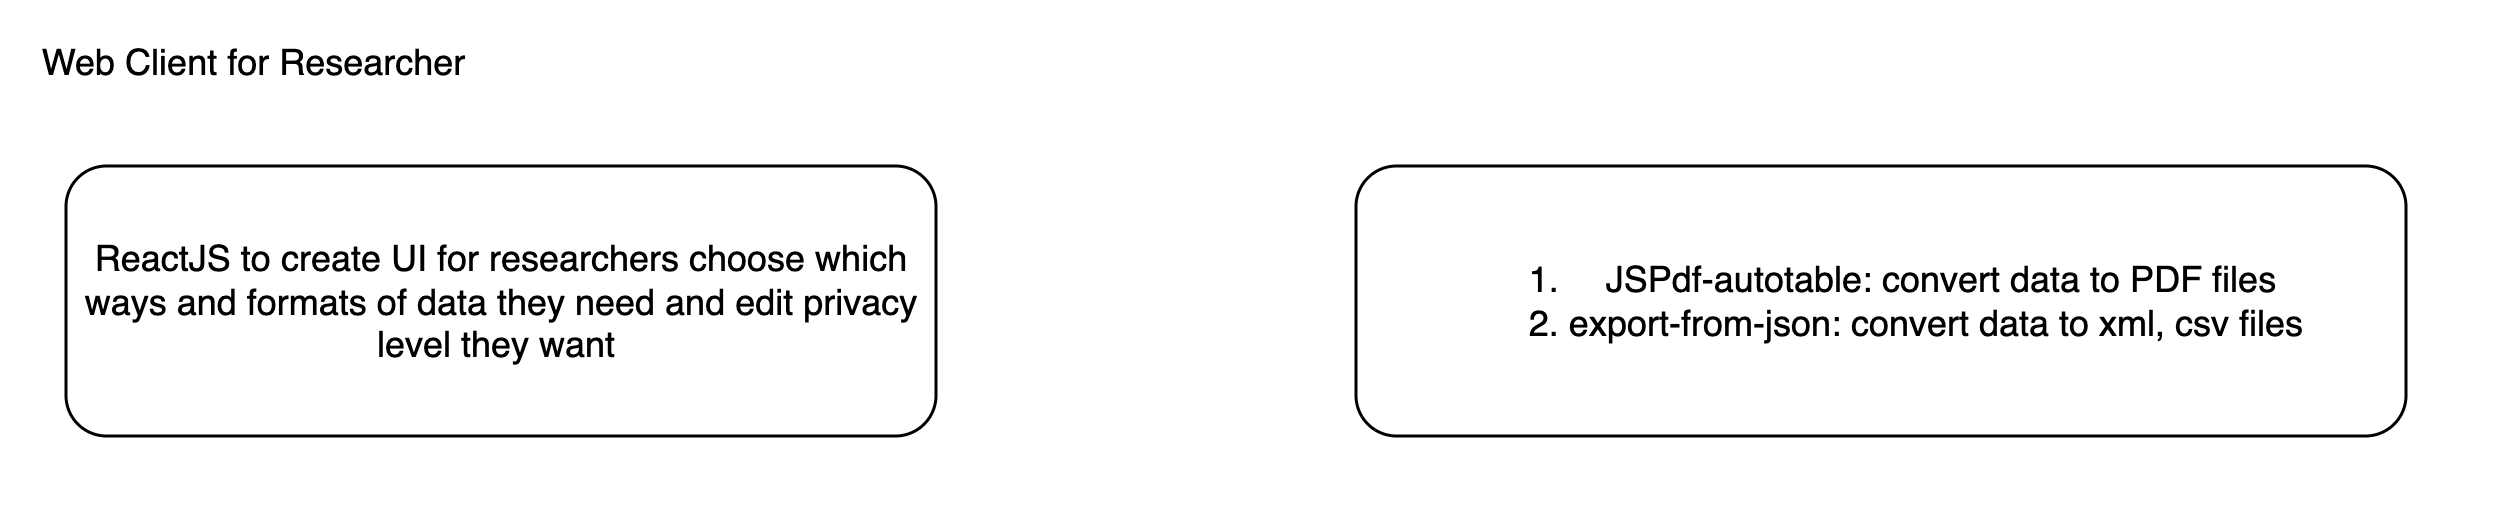
\includegraphics[width=16cm]{background_report/figures/web-system.png}
\caption{IMOTION Web System}
\label{figure:4}
\end{figure}

\subsection{Backend Service Design (Figure \ref{figure:5})}
The IMOTION backend service adopts a microservice architecture that boasts robust security, high availability, and scalability. Kubernetes automates the deployment and management of microservice applications, facilitating internal and external communication between services and users by exposing service ports. The Redis database is utilized for hotpot data caching. The Spring API Gateway serves as a reverse proxy, ensuring security measures and load balancing capabilities, while the PostgreSQL database cluster provides persistent data storage. Additionally, the design encompasses five key API microservices: User API handles user Data invocation; Data Collection API manages user-related data collection and invocation; Statistics and Survey API facilitates data processing and analysis; AI model contributes intelligence to the service; Researcher API enables researcher-related operations invocation. Google Apple Map Server supplies maps for the service. All communication takes place over HTTP to guarantee secure data transmission. This backend service is meticulously designed to meet modern Internet application requirements while delivering stable, efficient, and intelligent support.
\begin{figure}
\centering
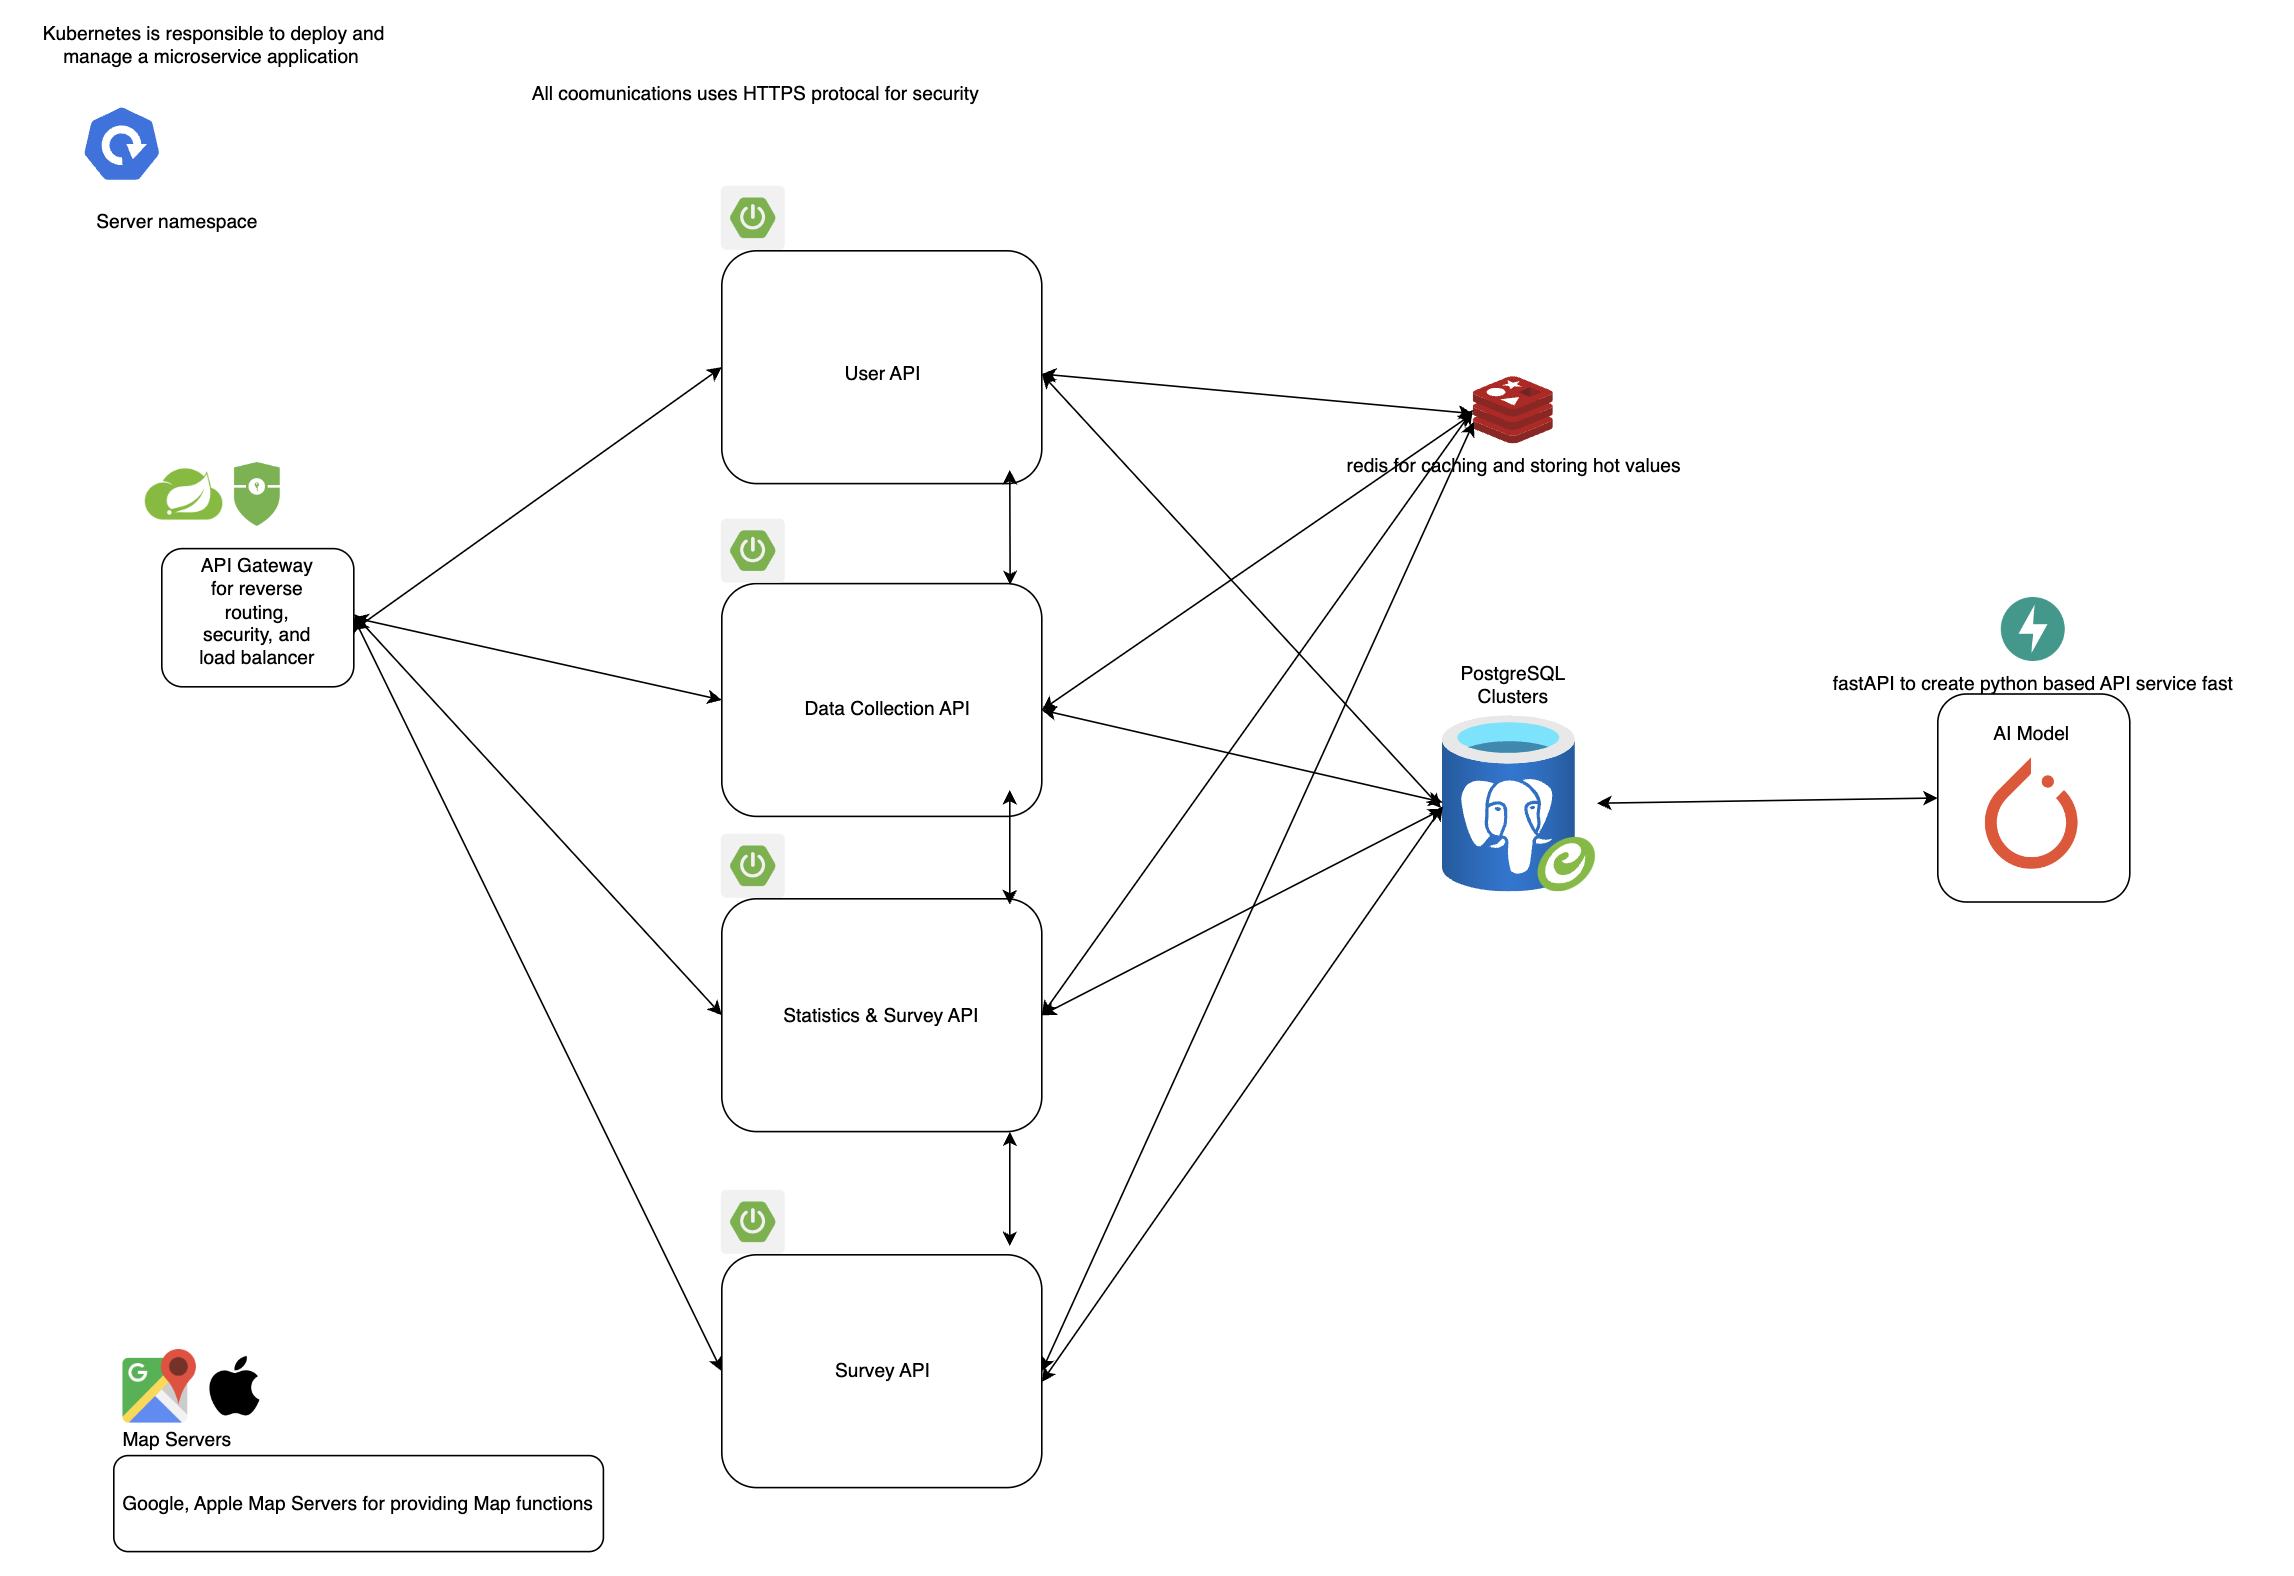
\includegraphics[width=16cm]{background_report/figures/backend-service-system.png}
\caption{IMOTION Backend Service System}
\label{figure:5}
\end{figure}
\section{Database Design}
\begin{itemize}
    \item General Entity, which contains information about application's users and what privacy level users want to participant. The interaction log describes how users interact with system.
    \item Raw Data is responsible for retrieving information from mobile devices or third-party APIs, including GPS data, acceleration measurements, health-related information, and energy usage in vehicles or homes. The acceleration data is utilized to predict the transportation modes used by the user during a trip.
    \item Activity Entity is responsible for storing a table containing information about the purpose of the activity or trip, where users can select their perceived purpose of the trip. There are two types of Trip entities: inference trips and ground-truth trips. Inference trips store user path segmentation predicted by machine learning models from raw data and predict the utilized traffic facilities. Ground-truth trips are modified by users based on their own memories to improve the model's accuracy.
    \item Researcher Entity stores researchers' information, with exclusive access granted to authorized researchers through the web-based management system. The privacy level is determined and stored by each researcher, allowing users to make personalized choices.
    \item The JWT-Session-Key Entity utilizes Redis to store critical data, such as authentication information and frequently accessed data.
\end{itemize}
\begin{figure}
\centering
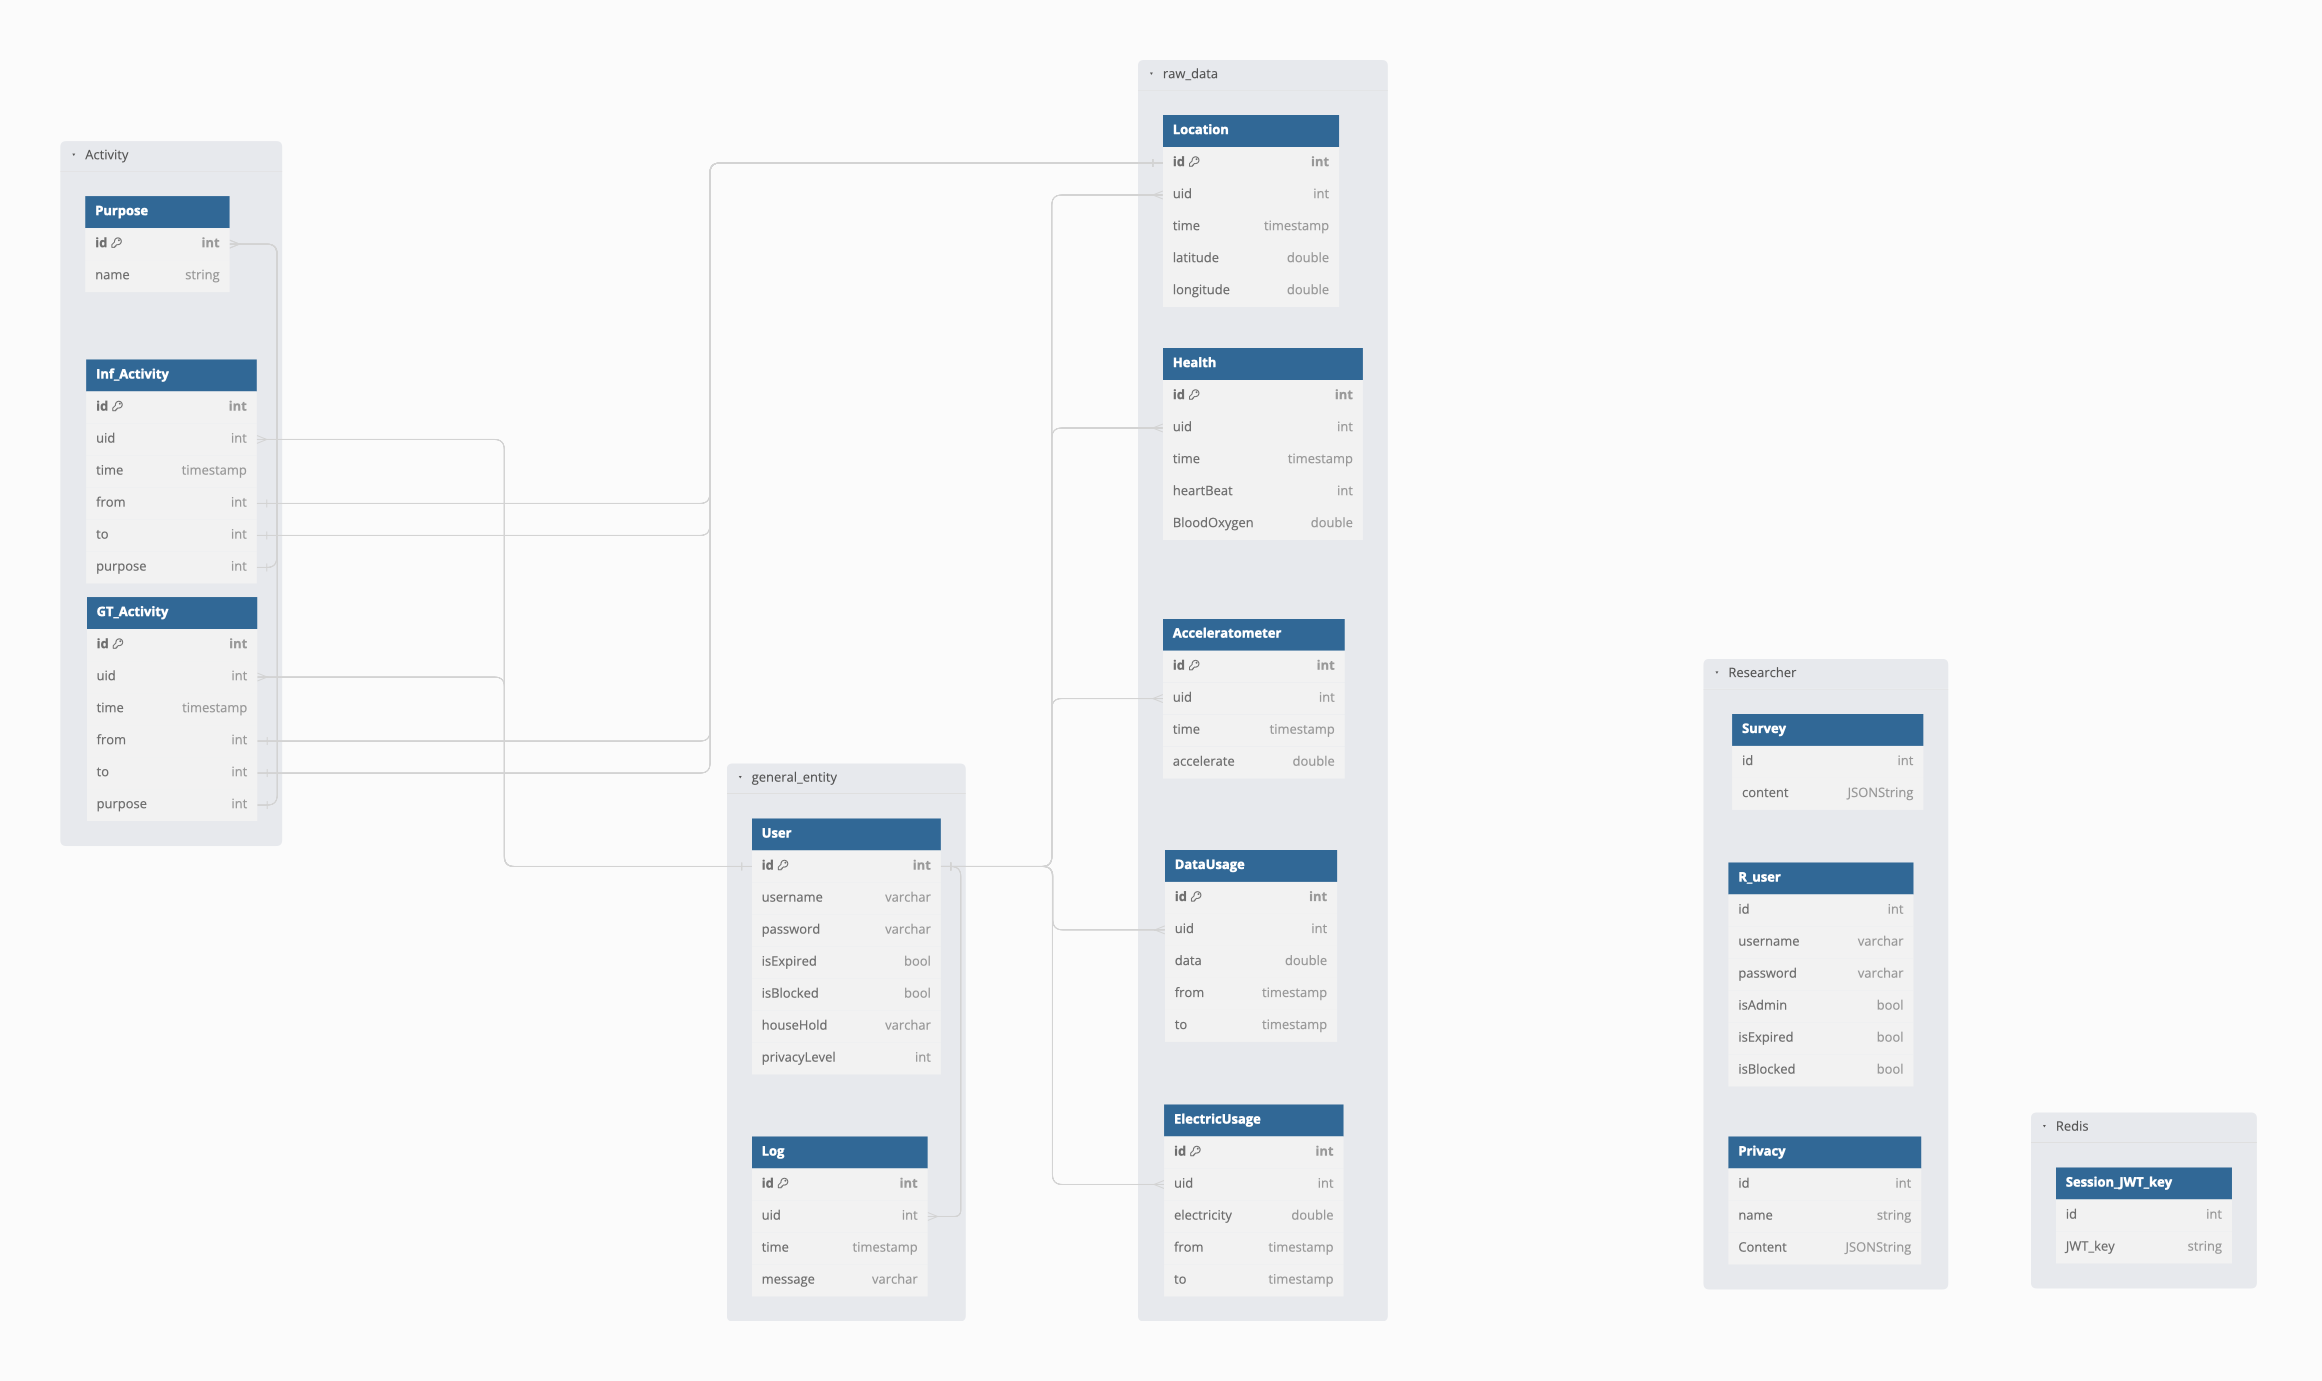
\includegraphics[width=16cm]{background_report/figures/database.png}
\caption{IMOTION Database Design}
\label{figure:6}
\end{figure}
\section{Machine Learning Design\cite{liang2019deep}}
For this application, I have implemented the machine learning model proposed by (Liang 2019). The model efficiently and accurately identifies various transportation modes solely based on accelerometer data from mobile phones. These recognized modes include stationary, walking, cycling, bus, car, subway, and train. In the experimental verification conducted in the paper, this model achieved an impressive accuracy of 94.48\%, surpassing traditional machine learning techniques. Notably, due to its reliance only on accelerometer data, it exhibits minimal resource consumption on the phone system.

\subsection{Data Processing}
\begin{enumerate}
    \item Data collection: This application determines the sampling frequency of the accelerometer based on user-defined privacy levels with a default setting of 50 samples per second.
    \item Gravity Subtraction: Considering Earth's gravity as a universal influence affecting all objects uniformly; we eliminate its impact using a low-pass filter since it is irrelevant for traffic pattern recognition.
    \item Data Smoothing: We employ the central moving average algorithm to process acceleration data effectively and reduce fluctuations caused by unexpected movements of mobile phones.
    \item Data Window Sliding: To enhance adaptability to changes in phone position and orientation, we utilize acceleration magnitude instead of specific axis data. Additionally, we segment time series data into fixed-size windows to meet real-time detection requirements.
\end{enumerate}

\subsection{Model Construction}
The paper presents a specialized convolutional neural network (CNN) (Figure \ref{figure:7} and \ref{figure:8}) for processing one-dimensional acceleration data, aiming to accurately identify users' transportation modes in different time periods.
\begin{enumerate}
    \item Input layer: The network receives a one-dimensional acceleration data vector with a scale of 512×1 per time window.
    \item Convolutional layers: Multiple convolution kernels are utilized to extract features from the input data. The first convolution layer consists of 32 convolution kernels sized at 15×1, and the convolution operation is performed with a step size of 1. Subsequently, the data undergoes dimensionality reduction through the Max pooling layer.
    \item Fully connected layer: After multiple convolution and pooling operations, the data is reduced to 8×64 and then fed into a fully connected layer that further compresses its dimensions to 200×1.
    \item Output layer: Finally, the transformed data becomes a 7×1 output vector representing probabilities associated with various transportation modes.
    \item Network features: This network employs convolution and pooling operations for feature extraction in acceleration data while utilizing the fully connected layer for classification purposes, enabling accurate detection of users' transportation modes. To enhance model convergence speed, Leaky ReLU is adopted as an activation function along with Adam optimization algorithm and L2 regularization techniques to prevent overfitting.
\end{enumerate}
\begin{figure}
\centering
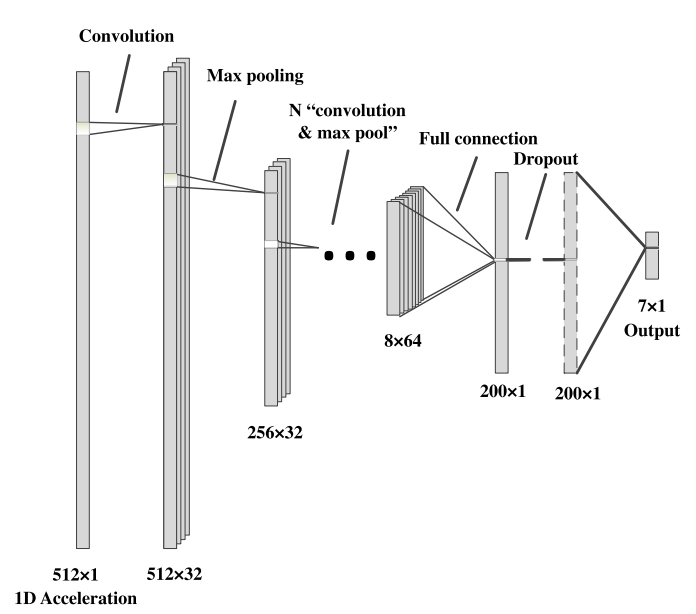
\includegraphics[width=16cm]{background_report/figures/model.png}
\caption{IMOTION Model Design\cite{liang2019deep}}
\label{figure:7}
\end{figure}

\begin{figure}
\centering
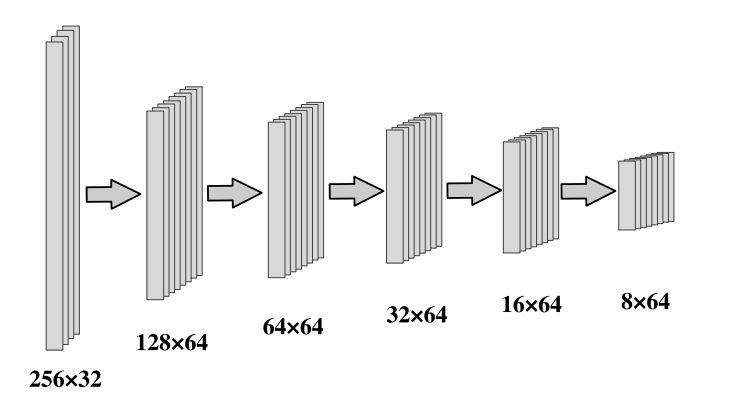
\includegraphics[width=16cm]{background_report/figures/hidden layer.png}
\caption{Hidden Layer Details\cite{liang2019deep}}
\label{figure:8}
\end{figure}
\section{Ethical Consideration}
This section will addresses the ethical and professional considerations taken into account during the development and evaluation of the project. Firstly, collecting and storing user information is a crucial issue. When users create profiles, they authenticate via email and provide personal information such as their name, occupation, home address, geolocation, and personal relationships. According to GDPR guidelines published by the UK Information Commissioner's Office (ICO), individuals have the right to be informed about how their personal data is collected and used \cite{ico2024}. Personal data refers to any information that can identify an individual, such as name or location \cite{icoPersonalInfo}. The IMOTION project adheres to these guidelines by clearly informing users of the purpose of data collection before they sign up. Additionally, Firebase service used in this project for phone authentication is GDPR compliant and has been audited against various privacy and security standards \cite{firebasePrivacy2024}. Protecting personal data is equally important when it comes to usability research. In end-user test surveys, only age range and device information were collected from participants to ensure anonymity without collecting identifiable information.\newline

Secondly, security and privacy issues related to GPS tracking and accelerometer data collection must also be handled with care \cite{ico2024}. The app activates GPS sensors only with explicit consent from users while displaying a real-time location-tracking pointer on its interface so that users are aware that their location information is being recorded.\newline

Finally, it is imperative to conduct rigorous scrutiny of algorithms, particularly in the context of machine learning APIs, in order to identify and mitigate any potential biases. It is crucial that technology ensures inclusivity and equity by delivering fair outcomes irrespective of gender, race, age or socioeconomic status\cite{ai2019high}. Simultaneously, transparency regarding the employed AI and machine learning models should be upheld through public availability of their decision-making processes and comprehensive documentation for review purposes. Furthermore, supporting external audits becomes essential to guarantee adherence to ethical standards\cite{icoAI}.
%% bibliography
\bibliography{background_report/references}



\end{document}
